% vim:spelllang=uk,en
\documentclass[simple,14pt,utf8,ukrainian]{eskdtext}
\usepackage{eskddstu}

\usepackage{cmap}
\usepackage[T2A]{fontenc}
\usepackage[utf8]{inputenc}
%\usepackage{concrete}
\usepackage{cite}
\usepackage{url}

\usepackage{textcase}

\usepackage{lscape}

\pdfcompresslevel=9 % сжимать PDF
\usepackage{pdflscape} % для возможности альбомного размещения некоторых страниц
\usepackage[pdftex]{hyperref}
% настройка ссылок в оглавлении для pdf формата
\hypersetup{unicode=true,
            pdftitle={Диплом},
            pdfauthor={Погода Михайло},
            pdfcreator={pdflatex},
            pdfsubject={},
            pdfborder    = {0 0 0},
            bookmarksopen,
            bookmarksnumbered,
            bookmarksopenlevel = 2,
            pdfkeywords={},
            colorlinks=true, % установка цвета ссылок в оглавлении
            citecolor=black,
            filecolor=black,
            linkcolor=black,
            urlcolor=blue}

\usepackage{amsmath}
\usepackage{amssymb}
\usepackage{moreverb}
\usepackage{indentfirst}
\usepackage{misccorr}

\usepackage{xtab}
\usepackage{nccfoots}
\usepackage{nccstretch}
\begin{document}
\ESKDstyle{empty}
\begin{titlepage}
  \thispagestyle{empty}
  \begin{center}
\large

Міністерство освіти і науки, молоді та спорту України

Національний технічний університет України

,,Київський політехнічний інститут''

\vspace*{1cm}

Факультет прикладної математики
\vspace*{2cm}

\textbf{Звіт з навчальної практики}

\vspace*{1cm}

на тему ,,Відновлення якості зображення за допомогою деконволюції''

\end{center}
\vspace*{1.5cm}

\normalsize
Місце проходження практики: \hfill кафедра ПМА, ФПМ, НТУУ <<КПІ>>\\

Керівник практики від підприємства: \hfill ас.~Терещенко~І.\,О.\\

Керівник практики від НТУУ,,КПІ'': 	\hfill ас.~Ковальчук-Хімюк~Л.\,О. \\

Виконав:\hfill Погода~М.\,В.\\

\hfill група КМ-92\\

Захищено з оцінкою:	\underline{\hspace{5cm}}
\vspace*{1cm}

``\underline{\hspace{0.6cm}}'' \underline{\hspace{3cm}} 2013 р.

\vspace*{2cm}
\begin{center}
\large
Київ

2013
\end{center}
\end{titlepage}
\tableofcontents
\clearpage
\section*{ВСТУП}
\addcontentsline{toc}{section}{ВСТУП}
  За сучасних умовах значну популярність набули цифрові зображення.
  Цифрові фотокамери є в більшості мобільних телефонах, ноутбуках та в іншій
  портативній техніці (не кажучи про власне фотоапарати).

  Одна з умов, що забезпечили таке поширення цієї техніки було те, що люди
  бажають зафіксувати на цифровому знімку якусь подію якнайшвидше.
  Зараз досить достати пристрій, натиснути кнопку й почати знімати.

  Одним з недоліків такого методу є те, що такі фотографії часто бувають
  не в фокусі або розмитті.
  Дуже часто немає нагоди перезняти такі невдалі кадри.

  Існують багато методів відновлення зображень, що дозволяють прибрати брак з
  фотографії.
  Одним з таких методів є операція зворотньої згортки, яка буде розглянута в
  цій роботі.
  \clearpage

\section{ПОСТАНОВКА ЗАДАЧІ}
  Необхідно розглянуті теоретичну основу відновлення зображення за допомогою
  деконволюції.
  Для цього необхідно розібрати поняття:
  \begin{itemize}
    \item цифровий сигнал;
    \item згортка, як математична операція;
    \item функція розсіювання точки;
    \item деконволюція, або обернена згортка, її види.
  \end{itemize}

  Необхідно розглянути існуючи методи, що дозволяють відновити зображення,
  коли відом сигнал, через який було отримане розмиття, а саме:
  \begin{itemize}
    \item Алгоритм Люсі"=Річардсона --- найпоширеніший ітеративний алгоритм;
    \item Алгоритм Вінера --- найпоширеніший неітеративний алгоритм.
  \end{itemize}
  \clearpage

\section{ТЕОРЕТИЧНІ ВІДОМОСТІ}
  \subsection{Поняття сигналів та їх згортки}
    \emph{Сигнал} --- зміна фізичної величини (наприклад, температури, тиску
    повітря, світлового потоку, сили струму тощо), що використовується для
    пересилання даних.
    Сигнали можуть бути:
    \begin{itemize}
      \item \textbf{одновимірними}: інфрачервоні спектри або звукові сигнали;
      \item \textbf{двовимірними}: цифрові зображення;
      \item \textbf{тривимірні}: зображення, отримані мікроскопом (так звані
        Z"=стеки);
      \item \textbf{многовимірні}: серії трьохвимірних сигналів, зняті у
        послідовні моменти часу
    \end{itemize}

    \emph{Згортка} --- операція, що показує ,,схожість'' однієї функції з
    відбитою та зрушеною копією іншої.
    В математиці, згортка --- це математична операція двох функцій $f$ і $g$, що
    породжує третю функцію, яка зазвичай може розглядатися як модифікована
    версія однієї з початкових.
    По суті, це особливий вид інтегрального перетворення:
    \[
      \left( f * g \right)\left( x \right) \stackrel{\mathrm{def}}{=}\
      \int_{-\infty}^\infty f(\tau)\, g(t - \tau)\, d\tau
    \]

    Через операцію згортки описуються багато деградацій, що зустрічаються на
    практиці:
    \begin{itemize}
      \item несфокусірованного розмиття;
      \item розмитість (наприклад, через струс камери);
      \item дифракційного розмиття;
      \item тощо.
    \end{itemize}
    \clearpage

  \subsection{Обернена згортка як метод відновлення}

    Процеси, спрямовані на те, щоби усунути деградації з сигналів (не лише тих,
    що обумовлені згорткою) називають процесами \emph{відновлення}.
    Одним з таких процесів є деконволюція.

    \emph{Деконволюція}, або \emph{обернена згортка} --- операція, що є
    оберненою до згортки двох сигналів.
    Можливість ,,пере"=фокусувати'' розмите зображення після того, як воно було
    зняте (використовуючи певні обрахунки) може бути надзвичайно корисним,
    наприклад, коли неможливо зняти заново фотографію.

    Деконволюція має за собою мету обернути деградації сигналів, що були
    отримані через операцію згортки.
    Існують й інші види деградацій, але обернена згортка, зазвичай, не в змозі
    допомогти із ними.

    Під час роботи з цифровим зображенням ми говоримо про відновленні зображення,
    або, більш конкретніше, об деконволюції зображення.
    Оскільки цей процес намагається отримати сигнал до того, як він зазнав
    певної деградації, маючи лише цей деградований сигнал, деконволюція може
    бути класифікована як \emph{зворотна задача}, а отже й математика зворотних
    задач тісно пов’язана з розумінням та розробкою алгоритмів деконволюції.

    \begin{figure}[!htb]
        \minipage{0.32\textwidth}
          
\includegraphics[width=\linewidth]{Aorig.png}
          \caption{Початкове зображення}\label{fig:orig-img}
        \endminipage\hfill
        \minipage{0.32\textwidth}
          
\includegraphics[width=\linewidth]{AOrig.jpg}
          \caption{Розмите зображення}\label{fig:conv-img}
        \endminipage\hfill
        \minipage{0.32\textwidth}
          
\includegraphics[width=\linewidth]{ADecon.jpg}
          \caption{Відновлене зображення}\label{fig:deconv-img}
        \endminipage\hfill
    \end{figure}

    Приклад роботи деконволюції зображення наведений на
    Рис.~\ref{fig:orig-img}--\ref{fig:deconv-img}.
    Як видно з цієї ілюстрації, процес оберненої згортки відновив багато
    деталей, що були ,,втрачені'' під час розмиття.
    Також треба звернути увагу на те, що відновлене зображення має певні
    цяточки, які були відсутні на початковому зображенні.
    Ці цяточки є прикладом \emph{артефактів} (небажаним ,,побічним ефектом'')
    деконволюції.\cite{deconvolve-index}
    \clearpage

  \subsection{Функція розсіювання точки та згортка}
    Оскільки деконволюція є оберненим процесом до згортки, для розуміння
    процесу оберненої згортки треба розуміти сам процес згортки.
    Власне кажучи, згортка --- це процес, що певним чином ,,змішує'' два
    сигнали.
    Кожна точка першого сигналу (назвемо його $f$) перероблюється у копію
    другого сигналу (назвемо його $h$).
    Кожна така копія має загальну інтенсивність таку, що дорівнює
    інтенсивності початкової точки сигналу $f$.
    Усі ці копії накладаються одна на одну, отримуючи таким чином сигнал $g$,
    що є згорткою сигналів $f$ та $h$.

    \begin{figure}[!htp]
      \centering
      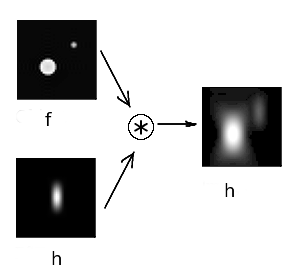
\includegraphics{conv.png}
      \caption{Приклад згортки}
      \label{fig:exconv}
    \end{figure}

    Саме тому операція згортки також відома як \emph{суперпозіціонний
    інтеграл}, а обернена операція --- \emph{розділенням сигналів}.
    Сигнал $h$ називають \emph{функцією розсіювання точки} (англ. Point Spread
    Function, або PSF), адже він визначає, як саме кожна точка сигналу $f$
    ,,розсіюється '' в копію PSF.
    Але згортка є комутативною операцією --- ми можемо визначити сигнал $f$ як
    PSF для сигналу $h$:
    \[ f * h = h * f \]
    Таким чином, згортка є особливою та відносно простою математичною
    операцією, а тому це досить примітно, що так багато деградацій, що
    зустрічаються повсякденно, можуть бути описаними за допомогою однієї й
    тієї ж самої операції.

    В вищенаведеному описі операції згортки було допущено, що однакова PSF
    була застосована до всіх точок сигналу $f$.
    Це припущення має місце в багатьох теоретичних викладках і має назву
    \emph{згортки з інваріантною у просторі функцією розсіювання точки}.
    Але в реальних ситуаціях має місце зміна (найчастіше поступова) PSF з
    переміщенням по сигналу $f$.
    Такий випадок називається \emph{згорткою зі змінною у просторі PSF}.
    В таких ситуаціях треба використовувати інші алгоритми деконволюції для
    відновлення зображення.\cite{book2}
    \clearpage
  \subsection{Види деконволюції}
    Деконволюцію можна класифікувати за інформацією, що відома про функцію
    розсіювання точки:
    \begin{itemize}
      \item \emph{Несліпа}.
        У цьому випадку PSF відома заздалегідь.
      \item \emph{Сліпа}.
        У цьому випадку функція розсіювання точки не відома заздалегідь, а
        тому потрібно використовувати інші методи відновлення зображення.
        Ця задача є набагато складнішою за несліпу деконволюцію, адже
        необхідно знайти оригінал зображення лише за деградованим зображенням.
        Для того, щоб рішення цієї задачі було можливим необхідно вказати
        певні межі можливого розв’язку.
        Насправді, вказувати межі може бути необхідно й при вирішенні задачі
        несліпої деконволюції, адже часто існує багато різних розв’язків.
      \item Випадки, коли відома частина PSF.
    \end{itemize}
    \clearpage

  \subsection{Взаємозамінність згортки та деконволюції}
    Операція згортки не завжди пов’язана з деградацією сигналу.
    Насправді, за допомогою ,,правильної'' PSF, згортка може прибрати розмиття
    зображення, а також проста згортка з так званим \emph{зворотним фільтром}
    може фактично зробити деконволюцію попереднього перетворення.

    Таким чином, згортка та деконволюція при певних умовах можуть виконувати
    однакові дії.
  \clearpage
\section{Алгоритми деконволюції}
\subsection{Алгоритм Річардсона-Люсі}
  Цей алгоритм дозволяє відновити зображення, що було розмите відомою
  функцією розсіювання точки.

  Точки розмитого зображення можуть бути представленими у формі суми:
  \[ d_i = \sum_j p_{ij} u_j, \]
  де $p_{ij}$ --- частина інтенсивності, що розсіялася з позиції $j$ в
  позицію $i$, $u_j$ --- $j$-та точка зображення, $d_i$ --- $i$-та точка
  отриманого розмитого зображення.\cite{richardson-hadley}

  Головна ідея полягає в тому, що необхідно підрахувати найбільш"=вірогідне
  значення $u_j$, якщо відомі $d_i$ та $p_{ij}$.

  \begin{equation}
    u_j^{(t+1)} = u_j^{(t)} \sum_i \frac{d_i}{c_i} p_{ij}
    \label{eq:rl-deconv}
  \end{equation}

  \[c_i = \sum_j p_{ij} u_j^{(t)}\]
  \clearpage
\subsection{Алгоритм Вінера}
  Нехай дане рівняння
  \begin{equation}
    y(t) = h(t)*x(t) + n(t)
    \label{eq:w-start}
  \end{equation}

  У цьому рівнянні:
  \begin{itemize}
    \item $x(t)$ --- деякий вхідний (невідомий сигнал) в позиції t;
    \item $h(t)$ --- відомий відгук системи;
    \item $n(t)$ --- деякий шум, що не залежіть від $x(t)$;
    \item $y(t)$ --- вихідне (розмите) зображення.
  \end{itemize}

  Мета полягає в знаходженні певного сигналу $g(t)$, за допомогою якого б ми
  могли оцінити $x(t)$:
  \begin{equation}
    \hat{x}(t) = g(t)*y(t)
    \label{eq:w-idea}
  \end{equation}

  $\hat{x}(t)$ --- оцінка $x(t)$, така, що мінімізує середню квадратичну
  помилку.

  Деконволюція Вінера дозволяє знайти цей $g(t)$.
  Найпростіше вона описується в частотній області:
  \begin{equation}
    G(f) = \frac{H^*(f)S(f)}{ |H(f)|^2 S(f) + N(f) }
    \label{eq:w-filter}
  \end{equation}
  Де:
    \begin{itemize}
      \item $G(f)$ та $H(f)$ --- сигнали, що були отримані за допомогою
        перетворення Фур’є з сигналів $g(t)$ та $h(t)$ відповідно;
      \item $S(f)$ --- середня спектральна щільність інтенсивності вхідного
        сигналу $x(t)$;
      \item $N(f)$ --- середня спектральна щільність шуму $n(t)$.
    \end{itemize}

  Сама фільтрація може бути проведена саме у просторі частот:
  \[
    \hat{X}(f) = G(f)Y(f)
  \]
  Де $\hat{X}(f)$ --- перетворення Фур’є від сигналу $\hat{x}(t)$, а тому
  можливо знайти $\hat{x}(t)$ застосувавши обернене перетворення Фур’є.
  \clearpage

\section{ВИСНОВКИ}
Під час огляду зазначеного матеріалу було з’ясовано, що операція згортки
дуже часто використовується при обробці сигналів (звукових, електричних;
одновимірних та багатовимірних), а тому може вважатися одною з основних
операцій у цьому напрямку.

Багато різних перетворень сигналів описується через згортку, проте
обернена операція може бути досить нетривіальною.

Складність цієї задачі змінюється зі збільшенням розміру зображення,
варіативності функції розсіювання точки, тощо.

Були розглянуті два найпоширеніших алгоритми деконволюції, ітеративний та
неітеративний.
Ітеративний використовує менш затратні обчислення, ніж алгоритм Вінера,
але може потребувати багато ітерацій.
Алгоритм Вінера використовує перетворення Фур’є, а тому математичний
апарат, необхідний для його реалізації є складнішим за той, що необхідний
для алгоритму Люсі"=Річардсона.


\bibliographystyle{ugost2008ls}
\bibliography{src}
\end{document}
